Interactions between electrons in solids can be treated broadly in two different ways, depending on the strength of the interaction.
Let us start with the case where the interactions are weak compared to their kinetic energy.
In this case, interactions may be treated as a perturbation
\begin{equation}\label{eq:interactionhamiltonian}
V = \sum_{\vec{p}\vec{p}'\vec{q},\sigma\sigma'}V(\vec{q})c^\dagger_{\vec{p}+\vec{q},\sigma}c^\dagger_{\vec{p}'-q,\sigma'}c_{\vec{p}',\sigma'}c_{\vec{p},\sigma}
\end{equation}
on top of the usual hamiltonian
\begin{equation}\label{eq:kinetichamiltonian}
H_0 = \epsilon_{\vec{p}} c^\dagger_{\vec{p},\sigma}c_{\vec{p},\sigma}
\end{equation}
for the noninteracting electrons.
The key insight, due conceptually to \citet{landau_theory_1957} and later formalized by \citet{gell-mann_bound_1951}, is that, as long as the interactions are sufficiently weak, this problem can be adiabatically connected to a similar problem with non-interacting quasiparticles.
Since these quasiparticles are fermions, they obey the Pauli exclusion principle, and the phase space available for scattering low-energy excitations thus goes to zero at small energies.
By Fermi's golden rule, the lifetime of such particles thus approaches infinity as we get closer and closer to the Fermi surface; i.e., there are still well-defined quasiparticles there.
Such a system is hence referred as a ``Fermi liquid,'' to signify the fact that we have made only a slight departure from the nominal model of a Fermi gas where the particles are treated as noninteracting.

Fermi liquid theory is unreasonably successful in describing the ground state of correlated electron systems.
Truly \emph{most} metals can be very adequately described as a simple Fermi gas with renormalized effective mass, specific heat, etc.; while these modifications may be large (e.g. $m^*/m\approx\num{e3}$ in \ce{CeAl3}), they otherwise look like normal metals.
Nevertheless, we can discuss circumstances in which the theory fails.
Clearly various electronic instabilities may gap out the Fermi surface, resulting in an insulator; this happens for arbitrarily weak interactions in quasi-\oned systems due to the Peierls mechanism, and in higher dimensions due to, e.g., Fermi surface nesting.
Whether the interaction is attractive or repulsive determines whether the instability occurs in the charge or the spin channel.
In the other limit, where the kinetic energy hamiltonian \ref{eq:kinetichamiltonian} is treated as a perturbation to the interaction term \ref{eq:interactionhamiltonian}, the Fermi liquid state gives way to an (Mott, or Wigner) insulating state where the electrons become localized so as to minimize the coulomb repulsion $U$.

Studying such departures from Fermi liquid theory has become one of the most important fields in condensed matter physics.
It is usually referred to as ``strongly correlated electron physics'', but many of the instabilities mentioned above are present even in the limit of weak interactions.
Much of this interest was spurred by the discovery in \num{1986} by \citet{bednorz_possible_1986} of high-$T_c$ superconductivity in \ce{Ba_xLa_{5-x}Cu5O_{5(3-y)}}, although the field has grown to include many other phenomena which occur in the strongly interacting limit that may or may not be related to superconductivity.
Despite nearly four decades of research, however, there still exists no universal theory for strongly correlated electron systems, in the sense that, if someone hands you a random strongly correlated material, it is impossible from the outset to \emph{predict} its ground state or its low-energy excitations.
In fact, it is not even clear such a theory ought to exist\citep{alexandradinata_future_2022}.

The \emph{field} of strongly correlated physics is thus, in some sense, still very much in its infancy, although that's not to say there haven't been huge advances, both theoretically and experimentally, especially since the discovery by \citet{bednorz_possible_1986}.
A lot of the effort experimentally has been focused on cataloguing the huge number of different exotic ordered phases---charge density wave, spin density wave, superconducting, strange metals, spin liquids, pseudogap, etc.---that are realized in these systems.
Usually this is done by mapping out a \emph{phase diagram} for each given material, which indicates which phases are present at various values of external parameters (magnetic field, pressure, strain, etc).
Ultrafast optics has played an important role in this respect, as it allows one to add a \emph{nonequilibrium} axis to such phase diagrams.
Such experiments, for example, have not only helped illustrate the extent to which different phases compete with one another in the cuprate phase diagram, but also the extent to which the action of the light pulse in strongly correlated materials can be used to tune the properties of those materials for practical purposes.
This is paradigm is referred to as ``ultrafast control,'' and I will discuss it in more detail in \cref{sec:ultrafastcontrol}.

A parallel effort in the field of ultrafast optics is to use the pump not to control the state of the material, but rather to excite coherent oscillations of the low-energy collective modes and study these oscillations in the time domain.
This approach is advantageous for two reasons.
For one, the frequencies accessible with this technique are bounded from below only by the length of one's delay stage, in contrast to conventional spectrometer-based methods which involve finite-frequency filters and gratings.
Second of all, the ability to select both the excitation mechanism (the pump) and the measurement apparatus (the probe) allows one to design experiments that target specific degrees of freedom of interest.
Thus, for example, in multiferroics, one can use \gls{shg} to selecitively probe the collective modes which modulate the macroscopic polarization.
This direction is referred to as ``ultrafast spectroscopy,'' which I will explain in detail in \cref{sec:ultrafastspectroscopy}.

This chapter may thus be regarded as an introduction to ultrafast optics, with special emphasis on how we can use ultrafast experiments to understand correlated materials without having to consider the interaction terms explicitly.
A complete review of this material is beyond the scope of this thesis; instead, I will focus on a few seminal works that I think tell this story most pedagogically.
Where appropriate, I point to pedagogical references that may be more useful than this thesis for these and other concepts.

\section{Spectroscopy}\label{sec:ultrafastspectroscopy}

\subsection{Collective modes}

The low-energy excitations of any many-body system are typically \emph{collective}, in the sense that they involve motion of all of the particles in the system rather than just one.
Let us consider, for example, the classical model consisting of two identical coupled harmonic oscillators
\begin{equation}
H = \sum_{i=1}^2\left(\frac{p_i^2}{2m}+\frac{m\omega_0^2}{2}x_i^2\right)+gx_1x_2,
\end{equation}
with mass $m$, natural frequency $\omega_0$, and coupling constant $g$.
When $g=0$, the normal modes of this system are simply the independent oscillation modes of the two oscillators.
However, for any nonzero $g$, the normal modes involve either symmetric or antisymmetric linear combinations of the two oscillator coordinates; that is, they involve collective motion of the two oscillators.
The extension to an ensemble of harmonic oscillators is straightforward; there, too, the normal modes of the Hamiltonian involve collective motion of all of the coordinates at once.

Of course the solids that we are interested in are more complicated than a simple ensemble of harmonic oscillators.
Usually, though, more complicated systems can be broken down into a small number of \emph{subsystems} which may, as a first approximation, be treated separately.
Thus, for example, it makes sense to refer to the phonon subsytem independently from the electronic subsystem, with different and independent collective mode spectra in the limit where the inter-subsystem coupling goes to zero.

When this coupling is finite, however, many interesting phenomena may occur.
For example, spin-orbit coupling---which implies a coupling between spin and orbital degrees of freedom of the electron---can, in the right circumstances, cause the statically ordered state of the spin subsystem to also induce a ferroelectric distortion of the electron orbitals.
The normal modes of the system in the presence of this coupling are no longer pure magnon or orbital modes, but rather collective modes of the spin and orbital degrees of freedom together.
Let us look at this phenomenon from a different perspective.
Suppose we didn't know the ground state of the system, but we did know that the relevant low-energy excitations involved both spin and orbital degrees of freedom (for example, we might see a response in both the time-resolved kerr rotation as well as the \gls{trshg}).
This is good evidence that the ground state of the system involves this coupling to some extent.
Thus, we have learned something quite important about our system without doing anything but look at the low-energy collective excitations.

\subsection{Coherent oscillations}\label{sec:coherentoscillations}

Clearly understanding the low-energy excitations corresponding to a given ground state is a useful way to understand its properties.
So far, however, we have made no mention of how to \emph{probe} these excitations in pump-probe spectroscopy.
Let us consider the following Hamiltonian consisting of electrons $c_{\vec{k}\sigma}$ (with dispersion $\epsilon_{\vec{k}\sigma}$) and bosons $b_{\vec{q}}$ (with dispersion $\omega_{\vec{q}}$) interacting via some potential $V^\sigma_{\vec{k}\vec{q}}$
\begin{equation}\label{eq:electronlatticehamiltonian}
H = \sum_{\vec{k}\sigma}\epsilon_{\vec{k}\sigma}c^\dagger_{\vec{k}\sigma}c_{\vec{k}\sigma}
+\sum_{\vec{q}}\hbar \omega_{\vec{q}}b^\dagger_{\vec{q}}b_{\vec{q}}
+\sum_{\sigma\vec{k}\vec{q}}V^\sigma_{\vec{k}\vec{q}}\left(b_{\vec{q}}+b^\dagger_{-\vec{q}}\right)c^\dagger_{\vec{k}\sigma}c_{\vec{k}+\vec{q}\sigma}.
\end{equation}
The average lattice displacement is given by
\begin{equation}
\big<u(\vec{r})\big> \propto \sum_{\vec{q}}\left(\big<b_{\vec{q}}\big>e^{i\vec{q}\cdot\vec{r}}+\big<b^\dagger_{\vec{q}}\big>e^{-i\vec{q}\cdot\vec{r}}\right).
\end{equation}
Clearly, in order for us to have a macroscopic lattice displacement, we need to have a finite value for $\big<b_{\vec{q}}\big>$ and $\big<b^\dagger_{\vec{q}}\big>$, which is impossible if there are a definite number of phonons in the mode $\vec{q}$ (since $\bra{n}b_{\vec{q}}\ket{m}=0$ for $n=m$).
In contrast, if the wavefunction of the system consists of a coherent superposition of different phonon numbers, $\big<u(\vec{r})\big>$ may acquire a finite value.
One thematic example of such a wavefunction is the so-called ``coherent state'' of the quantum harmonic oscillator
\begin{equation}\label{eq:coherentstate}
\ket{\alpha_{\vec{q}}} = \sum_n \frac{\alpha^ne^{-z^2/2}}{n!}(b^\dagger_{\vec{q}})^n\ket{0},
\end{equation}
although the real wavefunction need not be fully coherent to have a nonzero average lattice displacement.

One can show (see \citet{kuznetsov_theory_1994}) that the equation of motion for the operator $D_{\vec{q}}\equiv \big<b_{\vec{q}}\big>+\big<b^\dagger_{-\vec{q}}\big>$ due to \cref{eq:electronlatticehamiltonian} is
\begin{equation}\label{eq:coherentoscillationwaveequation}
\frac{\partial^2}{\partial t^2}D_{\vec{q}}+\omega^2_{\vec{q}}D_{\vec{q}} = -2\omega_{\vec{q}}\sum_{\vec{k}\sigma}V^\sigma_{\vec{k}\vec{q}}\big<c^\dagger_{\vec{k}\sigma} c_{\vec{k}+\vec{q}\sigma}\big>,
\end{equation}
i.e., $D_{\vec{q}}$ obeys a second-order differential equation with an inhomogenous part related (in this case) to the electronic subsystem.\footnote{There will also be a damping term, which may be added phenomenologically but is otherwise not considered in this treatment.}
Thus, if we manage to initialize a wavefunction with a finite $D_{\vec{q}}$, the frequency with which $D_{\vec{q}}$ oscillates in time is the frequency $\omega_{\vec{q}}$ of the boson $b_{\vec{q}}$.

The central idea in ultrafast spectroscopy is therefore to excite coherent modes like \cref{eq:coherentstate}, and then measure the frequency, damping, etc. of these modes by measuring $D_{\vec{q}}$.
This is in contrast to equilibrium spectroscopies, which measure, for example, the transfer of energy from the light field to states with a definite number of bosons (i.e., $\ket{n}\rightarrow\ket{n+1}$).
In theory, of course, the information obtained is the same---the frequency and damping coefficient of the collective modes in question may readily be optained in the equilibrium spectroscopies as well as in the pump-probe scheme.
\begin{enumerate*}[label=(\roman*)]\item[] However, as I argued at the start of this chapter, the pump-probe techniques offer a number of advantages, most notably \item the ability to design the pump and the probe to specify exactly which excitations we would like to measure, and \item the ability to measure much lower frequencies than in conventional spectroscopy due to the energy being measured in the time domain, rather than the frequency domain.\end{enumerate*}

\subsection{Excitation mechanisms}

The next question is: how do we intend to excite these coherent oscillations in real materials?
The truth is there are many such mechanisms; however, we can start by placing them into two generic categories.
\emph{Impulsive} mechanisms involve using the light pulse to apply an effective force to the relevant degrees of freedom in the material, which lasts for the duration of the light pulse; i.e., it is a delta function in time.
\emph{Displacive} mechanisms are, in contrast, typically a step function; i.e., the equilibrium position of the oscillator is different before and after the light pulse.
One important experimental difference is that impulsive excitation results in a coordinate $D_{\vec{q}}(t)\propto\sin(\omega t)$, whereas displacive excitation results in $D_{\vec{q}}(t)\propto\cos(\omega t)$; this can be seen simply by solving
\begin{equation}\label{eq:Dqequationofmotion}
\frac{\partial^2}{\partial t^2}D_{\vec{q}}+\omega^2_{\vec{q}}D_{\vec{q}} = f(t)
\end{equation}
for $f(t)\propto \delta(t)$ or $f(t)\propto \theta(t)$, respectively.

\subsubsection{In absorption}

Let us consider the Hamiltonian in \cref{eq:electronlatticehamiltonian}.
We saw that this Hamiltonian resulted in an equation of motion given by \cref{eq:coherentoscillationwaveequation}, which is a differential equation for $D_{\vec{q}}$ with an inhomogenous part
\begin{equation}\label{eq:electronlatticeforceterm}
f(t) = -2\omega_{\vec{q}}\sum_{\vec{k}\sigma}V^\sigma_{\vec{k}\vec{q}}\big<c^\dagger_{\vec{k}\sigma} c_{\vec{k}+\vec{q}\sigma}\big>,
\end{equation}
where the time-dependence of the right hand side is complicated but may be phonemnologically modeled.
For example, let us suppose that we are in a semiconductor and that photon energy of our pump pulse is greater than the band gap of the material.
Thus, the action of the pump is to excite electrons from the valence band into the conduction band.
On a very fast timescale (\num{0.1}--\qty{10}{fs}) these electrons thermalize with themselves via electron-electron scattering, resulting in a quasi-equilibrium carrier distribution in which electrons and holes have settled at the bottom of the conduction band and the top of the valence band, respectively.
Since further decay of these excitations is gapped, the relaxation of this state back to equilibrium may be much longer than the pulse width, especially if the gap is indirect; thus, together with the assumption that the lattice dynamics happen on much longer timescales than the electron thermalization time, it is appropriate to model the force term in \cref{eq:electronlatticeforceterm} as a step function in time
\begin{equation}
f(t) \propto \begin{cases} 0 & t<0\\1 & t\ge 0 \end{cases}.
\end{equation}

Thus we have the generic result that above-gap excitation typically excites coherent oscillations \emph{displacively}.
In the case that the bosons of \cref{eq:electronlatticehamiltonian} are phonons, this is known as \gls{decp}, and was studied by many authors, notably \citet{zeiger_theory_1992}.
An important insight which follows from \cref{eq:electronlatticeforceterm} is that, in the limit where the quasi-equilibrium electron distribution doesn't break any symmetries of the original hamiltonian, the applied force also does not break any symmetries.
Thus only totally-symmetric phonons may be excited via \gls{decp}.

\subsubsection{In transparency}\label{sec:intransparency}

While the \gls{decp}-like mechanisms tend to dominate when the photon energy is above the band gap, they are forbidden in transparency.
In this case, the dominant excitation mechanism is usually impulsive.
To see this, let us consider the case of a collective mode with energy $\hbar\omega_0$ which we wish to excite coherently with a below-gap ultrafast laser pulse.
If the central frequency of the light pulse is resonant with the collective mode (i.e., we have $\nu_\mathrm{photon}=\hbar\omega_0$), then we may drive the coherent oscillation directly; i.e., the mode coordinate $Q$ simply follows the electric field.
This is of course only possible if the mode carries a finite dipole moment (i.e. it is odd under parity).
Alternatively, we will see that, under the right conditions, we can also excite coherent oscillation of low-energy collective modes even if the photon energy is far away from any direct resonance.

To see this, recall that ultrafast laser pulses always have a nonzero bandwidth, proportional to the inverse of the pulse width.
In a nonlinear optical effect known as \gls{dfg}, pairs of these frequencies may \emph{interfere} to produce electric field components at the difference frequency between the two members of the pair.
Thus, as long as the collective mode in question has a frequency less than approximately the bandwidth $\delta \nu_\mathrm{photon}$ of the incident light pulse, there will exist pairs of frequencies $(\omega_1,\omega_2)$ in that light pulse such that $|\omega_1-\omega_2|\approx\omega_0$.
This electric field will last for the duration of the light pulse, which may be treated as a delta function in time.
This phenomenon is referred to as \gls{isrs}.

Since the force is a delta function in time, the result indeed is an impulsive excitation where the coordinate $D_{\vec{q}}(t)\sim\sin(\omega_0t)$.
Unlike the direct excitation mechanism mentioned above, \gls{isrs} requires two photons and the force is thus even under parity; i.e., we can only excite even-parity bosons.

It is instructive at this point to consider \gls{isrs} in a phenomenological \gls{gl} model.
We start by writing down an effective free energy\citep{stevens_coherent_2002}
\begin{equation}\label{eq:isrsfreeenergy}
F = -\chi_{ij}E_i(t)E_j(t)Q
\end{equation}
where $\vec{E}(t)$ is the incident electric field, $Q$ the mode coordinate,\footnote{Here we treat the mode $Q$ as nondegenerate, although the generalization to the degenerate case is straightforward.} and $\chi_{ij}$ is some tensor of coefficients (see \cref{ch:shgtheory}).
The effective force $f$ due to \cref{eq:isrsfreeenergy} is
\begin{align}
f &= -\frac{\partial F}{\partial Q}\\
&= \chi_{ij}E_i(t)E_j(t)
\end{align}
which appears on the right hand side of \cref{eq:Dqequationofmotion}.
Clearly, if the $\vec{E}(t)$ has Fourier components $\omega_1$ and $\omega_2$ such that $|\omega_1-\omega_2|\approx\omega_0$, then the force will be \emph{resonant} with the oscillator frequency.

Some interesting insights may be made in light of \cref{eq:isrsfreeenergy}.
Let us consider for example the limit where the ``mode'' $Q$ is a static magnetization $M_k$.
The free energy reads\citep{juraschek_phono-magnetic_2020}
\begin{equation}
F = -\chi_{ijk}E_i(t)E_j(t)M_k,
\end{equation}
where we have expanded $\chi_{ij}$ to linear order in $\vec{M}$.
Then, there is an \emph{effective magnetic field}
\begin{align}
H^\mathrm{eff}_k &= \frac{\partial F}{\partial M_k}\\
&= \chi_{ijk}E_i(t)E_j(t)
\end{align}
which exists for the duration of the pump pulse.
This is the \gls{ife}, which may thus be thought of as a particular limit of \gls{isrs}.\footnote{Despite the similarities presented here, the two effects are actually quite different. For example, the spectral content of the pump pulse in the \gls{ife} does not change before and after interacting with the sample\citep{gridnev_phenomenological_2008}.}
A similar effect (known as the \gls{icme}) is also present; expanding $\chi_{ij}$ to second order in $\vec{M}$, we have
\begin{equation}
F = -\chi_{ijkl}E_i(t)E_j(t)M_kM_l
\end{equation}
and
\begin{align}
H^\mathrm{eff}_l &= \frac{\partial F}{\partial M_l}\\
&= \chi_{ijkl}E_i(t)E_j(t)M_k,
\end{align}
which, in contrast to the \gls{ife}, may occur when the pump is linearly polarized.
The \gls{icme} is also available in \glspl{afm}; writing
\begin{equation}
F = -\chi_{ijkl}E_i(t)E_j(t)L_kL_l,
\end{equation}
where $\vec{L}$ is the \neel vector (defined as the different in sublattice magnetizations), we have
\begin{align}
H^\mathrm{eff}_l &= \frac{\partial F}{\partial L_l}\\
&= \chi_{ijkl}E_i(t)E_j(t)L_k.
\end{align}
A full treatment of these and related effects is beyond the scope of this work;\footnote{See \citet{kirilyuk_ultrafast_2010} for a comprehensive review.} the point is just to draw a connection between the various impulsive excitation mechanisms available to us in ultrafast spectroscopy.

\subsection{Collective modes in correlated materials}

\subsubsection{Phase transitions and Goldstone's theorem}\label{sec:superfluidgoldstone}

In this section we illustrate one way we can understand the low-energy collective modes of a given material system without knowing precisely the form of the interaction Hamiltonian in \cref{eq:interactionhamiltonian}.
The important insight is that we can simply write down all of the \emph{symmetry-allowed} terms in the Hamiltonian (or, at nonzero temperature, the free energy), and examine fluctuations near a phase transition where some order parameter takes on a nonzero value.
In doing so, we find quite generally Goldstone's result that there is a gapless collective mode at the $\Gamma$ point for each spontaneously broken symmetry.
We also see that, in addition to the gapless Goldstone bosons, we also get a gapped \emph{amplitude} mode which may be measurable in certain circumstances.
The goal of this section is not to give a rigorous proof of Goldstone's theorem, but to illustrate how it comes about in a very simple model.

\begin{figure}
\centering
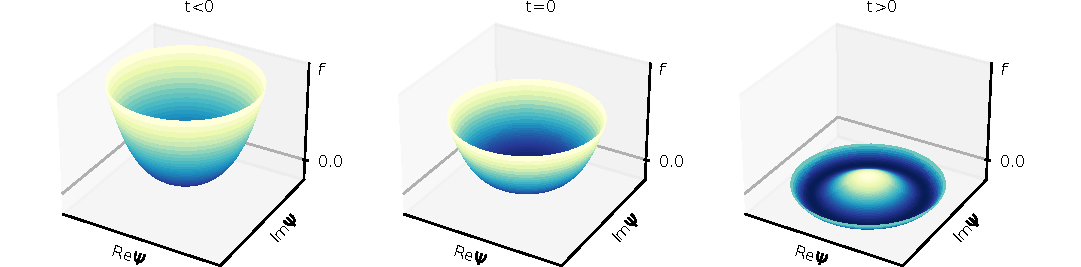
\includegraphics[width=0.8\textwidth]{gfx/ch1/pdf/glfreeenergydensity.pdf}
\caption[Schematic free energy density in the GL model.]{
\label{fig:glfreeenergydensity}
Schematic free energy density in the GL model.
}
\end{figure}

Let us consider the \gls{gl} free energy density in the case of superfluidity, which is a functional of the coarse-grained order parameter $\Psi(\vec{x}) \equiv \psi(\vec{x})e^{i\theta(\vec{x})}$ and whose lowest-order terms are
\begin{equation}\label{eq:glfreeenergydensity}
f[\Psi(\vec{x})] = -\frac{t}{2}|\Psi(\vec{x})|^2+\frac{u}{4}|\Psi(\vec{x})|^4+\frac{K}{2}|\nabla \Psi(\vec{x})|^2,
\end{equation}
where $u,K>0$ and $t=(T_c-T)/T_c$.
Clearly at all temperatures the minimum of \cref{eq:glfreeenergydensity} is spatially uniform, but for $T<T_c$ it occurs at a finite value of $\psi(\vec{x})$ (see \cref{fig:glfreeenergydensity})
\begin{equation}
\Psi(\vec{x}) = \overline{\psi} \equiv \sqrt{\frac{t}{u}},
\end{equation}
where we have (without loss of generality) set $\overline{\theta} = 0$.
Now consider fluctuations $\delta \theta(\vec{x})$ in the phase of the order parameter $\Psi$.
We have
\begin{equation}
f[\overline{\psi}e^{i\delta \theta}] = f[\overline{\psi}]+\frac{K\overline{\psi}^2}{2}|\nabla \delta \theta(\vec{x})|^2,
\end{equation}
where we have used that $-t+u\overline{\psi}^2=0$.
Let us write the fluctuation $\delta \theta(\vec{x})$ in terms of its Fourier transform
\begin{equation}
\delta \theta(\vec{x}) = \sum_{\vec{q}} e^{i\vec{q}\cdot\vec{x}}\delta \theta_{\vec{q}}.
\end{equation}
Then we have
\begin{equation}
F[\overline{\psi}e^{i\delta \theta(\vec{x})}] \equiv \int f[\overline{\psi}e^{i\delta\theta(\vec{x})}] \, d^3\vec{x} = F[\overline{\psi}]+\frac{KV\overline{\psi}^2}{2}\sum_{\vec{q}} q^2|\delta \theta_{\vec{q}}|^2.
\end{equation}
Thus, uniform ($\vec{q}=0$) fluctuations in the phase of $\Psi$ cost zero energy, and long-wavelength ($\vec{q}\approx0$) fluctuations in the phase of $\Psi$ cost very little energy.
The collective modes corresponding to these long-wavelength fluctuations are exactly our Goldstone modes.

Let us also examine the energy cost of fluctuations in the amplitude of $\Psi$, i.e. $\delta \psi(\vec{x}) \equiv \psi(\vec{x})-\overline{\psi}$.
To order $\delta \psi^2$, we have
\begin{equation}
f[\overline{\psi}+\delta\psi(\vec{x})] = f[\overline{\psi}]-\frac{t}{2}\delta\psi(\vec{x})^2+\frac{3u}{2}\overline{\psi}^2\delta\psi(\vec{x})^2+\frac{K}{2}(\nabla \delta \psi(\vec{x}))^2,
\end{equation}
and, inserting $\overline{\psi} = \sqrt{\frac{t}{u}}$,
\begin{equation}
f[\overline{\psi}+\delta\psi(\vec{x})] = f[\overline{\psi}]+\frac{t}{2}\delta\psi(\vec{x})^2+\frac{K}{2}(\nabla \delta \psi(\vec{x}))^2,
\end{equation}
so that (for $T<T_c$), even \emph{uniform} fluctuations in the amplitude of $\Psi$ cost nonzero energy.
The collective mode associated with such uniform fluctuations is the so-called ``amplitude'' or ``Higgs'' mode of our ordered superfluid, with the important result that the energy of this mode approaches zero for $T\rightarrow T_c$.

Observing the amplitude mode in real systems is challenging because its decay into the lower-energy Goldstone modes is not typically forbidden, and so its lifetime is usually too low to observe it as a true quasiparticle\cite{jain_higgs_2017}.
Nevertheless, amplitude modes have been observed in a number of different circumstances; mainly, of course, in superconductors, where the amplitude mode may appear as a Raman peak in the $A_{1g}$ channel\citep{measson_amplitude_2014}, but also in charge density wave\citep{wang_axial_2022} and magnetic\citep{hong_higgs_2017,jain_higgs_2017} systems (see \citet{pekker_amplitudehiggs_2015} for a good review).

\subsubsection{Example: electromagnons in multiferroics}

In the above we have described how coherent oscillations of collective modes in solids may be excited with an ultrafast laser, and we have explored how we can understand what those modes are without having to solve the full many-body Hamiltonian.
Let us start to apply this machinery to a relevant physical system.
A full accounting of the different collective modes in correlated systems is beyond the scope of this work; instead. let us focus on a particular class of physical system---multiferroics---which encompasses a lot of the physics of correlated materials and may also be described well in terms of the \gls{gl} theory we outlined above.
\Cref{ch:cubr2} is concerned with one member of this class (\ce{CuBr2}); in this material, we have evidence that the amplitude mode of the magnetic Hamiltonian is imprinted on the charge degrees of freedom in the form of an electromagnon.
The understanding developed here will thus be quite helpful when we encounter that chapter.

Multiferroics are materials in which magnetic order exists in the same phase as ferroelectric order.
They may typically be classified into two types.
In the so-called type-II multiferroics, the transition to the ferroelectric state appears at the same temperature as a concomitant magnetic transition.
This is because the ferroelectricity is \emph{due to} some inversion symmetry breaking of the magnetic order, for instance by a helical spin density wave.\footnote{The ferroelectricity is thus considered of the ``improper'' type.}
The microscopic mechanism will be discussed shortly, but let us contrast this with the case of type-I multiferroics---in type-I multiferroics, the magnetic and ferroelectric transition temperatures are different, and neither is ``due'' to the other; they just happen to exist in the same material.
Intuitively this may happen when magnetic ions exist alongside different ions which participate in the ferroelectricity; this is the case in \ce{BiFeO3}\cite{kiselev_detection_1963}.
Here we will focus on type-II multiferroics, not only because they tend to be more interesting but also because they usually have larger magnetoelectric effects (since the ferroelectric order is due to the magnetic order) and have thus been the central focus of the modern research on multiferroics.

The central question is then: can we describe (microscopically) how ferroelectricity may appear as a \emph{result} of long-range magnetic order?
A critical insight due to \citet{katsura_spin_2005} is that type-II multiferroicity can happen in quasi-\oned Mott insulators when spin-orbit coupling is strong and the spins are ordered in a \emph{magnetic spiral}.
\citet{katsura_spin_2005} consider a \num{3}-site \oned cluster model in which two transition metal ions with local spin-orbit coupled $d$ electron orbitals interact via superexchange across an intermediate ligand atom (with an associated set of $p$ orbitals).
The tendency towards magnetic ordering is put in by hand, by placing a local spin at each transition metal site $j$ in the direction $\hat{e}_j = (\cos\phi_j \sin\theta_j, \sin\phi_j \sin\theta_j, \cos\theta_j)$, and letting the $d$ spins $\vec{S}_j$ interact with these local spins via a Hamiltonian $H_U=-U\sum_j \hat{e}_j\cdot \vec{S}_j$.
They find quite generally the following geometrical relation between the spin directions $\hat{e}_j$ and an \emph{induced} polarization $\vec{P}$:
\begin{equation}\label{eq:knbtheoryequation}
\vec{P} \propto \hat{e}_{12}\times(\hat{e}_1\times\hat{e}_2)
\end{equation}
where $\hat{e}_{12}$ is the unit vector parallel to the bond connecting the two transition metal sites.

Clearly if $\hat{e}_1$ and $\hat{e}_2$ are either parallel or anti-parallel to one another, there is no induced polarization.
However, if the magnetic order is \emph{noncolinear}, and the spin plane is not perpendicular the chain direction, an induced polarization appears via \cref{eq:knbtheoryequation}.
This explains very generally the multiferroicity of many noncollinear magnets.
The multiferroic state thus described is also clearly ``type-II'', since the polarization is zero absent the magnetic ordering.
Heuristically, such a spiral magnetic order may occur due to competition between a ferromagnetic nearest neighbor exchange interaction $J_1$ and an antiferromagnetic next-nearest neighbor interaction $J_2$ in a \oned spin chain; for $|J_2/J_1|<4$ one can show that the ground state is such a noncollinear spiral.

Let us now consider the low-energy excitations of such a \oned chain.
The Hamiltonian may be written as
\begin{equation}\label{eq:knbhamiltonian}
H=H_1+H_2+H_3+H_4,
\end{equation}
where
\begin{equation}
H_1 = \sum_i J_1\vec{S}_i\cdot\vec{S}_{i+1}+J_2\vec{S}_i\cdot\vec{S}_{i+2},
\end{equation}
\begin{equation}\label{eq:knbpolarizationcoupling}
H_2 = -\lambda \sum_i \vec{u}_i\cdot [\hat{x}\times (\vec{S}_i\times\vec{S}_{i+1})],
\end{equation}
\begin{equation}
H_3 = \sum_i \frac{\kappa}{2}\vec{u}_i^2+\frac{1}{2m}\vec{P}_i^2,
\end{equation}
and
\begin{equation}\label{eq:knbanisotropy}
H_4 = \sum_i D(S^z_i)^2.
\end{equation}
This Hamiltonian describes a \oned spin chain along $\hat{x}$ interacting with a charge coordinate $u_i$ (with conjugate momentrum $P_i$) via \cref{eq:knbtheoryequation}.
The anisotropy $D>0$ pins the magnetic order to the $xy$ plane.
As discussed above, for $|J_2/J_1|<4$ the ground state is a noncollinear spin spiral with spins lying in the $xy$ plane, and the relative angle between adjacent spins is defined by some quantity $\phi\neq 0,\pi$ which is chosen to minimize the competition between $J_1$ and $J_2$.

\citet{katsura_dynamical_2007} discuss the low-lying excitations of this ground state in light of \cref{eq:knbhamiltonian}.
First of all, clearly uniform rotations of all of the spins in the chain cost zero energy; this is the \emph{Goldstone mode} of \cref{eq:knbhamiltonian}, and is in direct analogy with the Goldstone mode of the superfluid discussed in \cref{sec:superfluidgoldstone}.

If we temporarily set $D\rightarrow 0^+$ in \cref{eq:knbanisotropy}, we may also observe that, in this limit, uniform rotations of the spin spiral \emph{about the chain axis} also cost zero energy.
This mode is also a Goldstone mode, although in this case it is due to the spontaneous breaking of the $\hat{x}$ rotational symmetry rather than the $\hat{z}$ rotational symmetry.
For nonzero $D$, this mode of course acquires a finite energy; it is thus referred to as the \emph{pseudo}-Goldstone mode, to highlight the fact that the symmetry is explicitly broken by the Hamiltonian rather than spontaneously broken.

The pseudo-Goldstone mode, however, is still quite interesting---note that, due to \cref{eq:knbpolarizationcoupling} and \cref{eq:knbtheoryequation}, a rotation of the spins about the chain axis \emph{also} rotates the induced polarization about that axis.
This mode is thus our first encounter with an electromagnon, which is any spin boson that acquires a finite electric dipole moment due to coupling to the charge degrees of freedom.

Electromagnons are in fact an intrinsic feature of multiferroics, and what we have discussed above is by no means the only mechanism by which such modes may be achieved.\footnote{For example, in cases where magnetoelastic coupling is strong, a multi-particle excitation in which a spin boson couples to a phonon, and a phonon then couples to the electric polarization, is possible and common\citep{takahashi_magnetoelectric_2012}.}
While a complete description of electromagnons and multiferroics is beyond the scope of this work (see \citet{cheong_multiferroics_2007} and \citet{fiebig_evolution_2016} for review), I hope to have nevertheless motivated the idea that elementary excitations in correlated systems may still be understood in the context of broken symmetries and the \gls{gl} paradigm---a notion that we will encounter frequently in the course of this thesis.

\section{Control}\label{sec:ultrafastcontrol}

From a technological perspective, ultrafast spectroscopy is useful because it helps us understand the physics of materials in equilibrium and how those materials might function in practical applications.
Ultrafast control is different in the sense that it seeks to understand the different ways we can \emph{manipulate} materials, with the idea that the knowledge thus gained may be used as a control scheme in some future technology, whether that involves using light or some other stimulus.
The material of study is thus of a different kind of importance in ultrafast control---we are more interested in the phenomenology of the light-matter interaction rather than the phenomenology of the material itself.
Usually the phenomenology of interest is, for example, being able to control the \emph{state} of the material (like the direction of a magnetization, or the presence of a charge density wave) using light.

In my view, ultrafast control schemes may be divided into two categories.
In one case, the dynamics following the light pulse are \emph{coherent}; that is, the light field, for instance, excites coherent oscillations (see \cref{sec:coherentoscillations}), and those coherent oscillations drive the system to a new state.\footnote{Here I take the view that simply exciting coherent oscillations (i.e. without a dynamical phase transition) is \emph{not} coherent control, but some may disagree with this point perspective, especially when the amplitude of such oscillations are large.}
In contrast, \emph{incoherent} dynamics do not involve coherent oscillations of any degrees of freedom; instead, the light is used to, for example, heat the material, or excite quasiparticles away from the Fermi surface.
This can also drive the material into a different (nonequilibrium) state, for example by quenching some \gls{lro} of the electrons near the Fermi surface, but the mechanism is qualitatively different from the coherent case.
We will discuss both cases below.

\subsection{Incoherent control}

\subsubsection{Heating across a phase transition}

The most basic level of ultrafast control is to use the light pulse simply to heat the material; if the initial and final temperatures lie below and above an equilibrium phase transition, then ultrafast control has been achieved.
This is a somewhat trivial mechanism, but it played an important part in early research on ultrafast control, especially in materials where dynamical phase control \emph{not} based on heating was rare or difficult (such as antiferromagnets\citep{kimel_laser-induced_2004}).
In addition, interactions between the sample area melted by the pump pulse and the surrounding unpumped area may cause interesting effects, such as magnetization reversal in ferromagnetic thin films due to the stray field of the unpumped sample volume\citep{ogasawara_submicron-scale_2009}.
We are more interested, however, in \emph{nonthermal} ultrafast phenomena---that is, dynamical phenomena which cannot be replicated quasi-adiabatically.

\subsubsection{Nonthermal melting}\label{sec:nonthermalmelting}

One example of such a phonemonon is the ultrafast quench (or ``nonthermal melting'') of some equilibrium order parameter via photoexcitation of electrons by the pump pulse.
Let us consider, for example, the case discussed briefly in the beginning of this chapter of a quasi-\oned Fermi liquid which becomes gapped by a periodic lattice distortion (i.e. via the Peierls mechanism).
The basis for this mechanism is that quasiparticles near the Fermi vector in the undistorted Fermi liquid decrease their energy when the gap is opened (via hybridization of folded bands), which happens at the expense of some energy gain associated with distorting the lattice away from its equilibrium configuration.
When light is incident on this system in the distorted phase,\footnote{Let us say that the pump photon energy is above the Peierls gap.} quasiparticles are excited \emph{away} from the top of the valence band, and the energy savings we gained by distorting the lattice disappears.
The system thus relaxes back to its previous configuration and we lose our periodic lattice distortion---the light pulse destroyed the \gls{lro}.

Note that this is referred to as a \emph{nonthermal} effect, even though for typical metals the quasiparticles experience an effective temperature change on the order of \qty{e3}{K}\citep{rethfeld_ultrafast_2002}.
Nevertheless, the dynamical phase transition we just described proceeds, by construction, via the creation of a \emph{nonequilibrium} distribution of photoexcited electrons, and in this sense it is nonthermal.
There is often difficulty encountered in \emph{proving} that the action of the pump is truly nonthermal.
Indeed, the existence of an ordered phase implies some finite temperature $T_c$ where that order is destroyed by equilibrium thermal fluctuations---it is the job of the experimenter to show that the laser pulse is not simply heating the material above this critical temperature.
This is obvious if the phenomenology following the quench (see the next section) is in any case not reproduced in equilibrium, but may also be shown (heuristically) by dividing the energy absorbed by the material from the pulse by the heat capacity.

\subsubsection{Formal model: time-dependent Ginzburg-Landau theory}

In describing many-body systems in the static limit, we have seen that it is useful to define a phenomenological model which captures the important physics (via a free energy density, an order parameter, etc.), rather than attempting to treat the inter-particle interactions explicitly.
An important concept justifying this practice is the idea of \emph{universality}, which states that, since the correlation length $\xi$ diverges as we approach the critical point, the physics near the critical point is governed not by the microscopic details of the system but rather by a small set of characteristic quantities like the spatial dimensionality of the system and the symmetry of the order parameter\citep{wilson_renormalization_1974}.
This means that to understand any \emph{complicated} system of a particular universality class, it suffices to study the \emph{simplest} system in that universality class, as long as we are close to the critical point.\footnote{The validity of the universality hypothesis away from criticality is not obvious, but is often heuristically assumed to be the case.}

In the dynamic limit, the idea of universality is still thought to apply (thus, for example, the wavevector- and frequency-dependent susceptibility $\chi(\vec{k}, \omega)$ is a homogenous function near the critical point), but the relevant parameters now include not just the spatial dimensionality and symmetry of the order parameter but also new characteristics, like the presence of conserved quantities, and Poisson-bracket relationships between those conserved quantities and the order parameter\citep{hohenberg_theory_1977}.
We are thus motivated, as in the static case, to consider \emph{simple models} for each universality class to derive the important limiting behavior---this is the \gls{tdgl} theory.
One such model, which is valid when there are no conserved quantities, is the so-called ``Model A'' equation of motion
\begin{equation}\label{eq:modelaequation}
\frac{\partial\psi(\vec{x}, t)}{\partial t} = -\Gamma \frac{\delta F}{\delta \psi(\vec{x}, t)}+\eta(\vec{x}, t),
\end{equation}
where
\begin{equation}
F = \int \left[-\frac{t}{2}\psi^2+\frac{u}{4}\psi^4+\frac{K}{2}|\nabla \psi|^2\right] \, d^d\vec{x}
\end{equation}
and $\eta$ is a Gaussian white noise source with zero mean and two-point correlation function
\begin{equation}
\big<\eta(\vec{x}, t)\eta(\vec{x}', t')\big>=2\Gamma \delta(\vec{x}-\vec{x}')\delta(t-t')
\end{equation}
chosen to satisfy the fluctuation-dissipation theorem.

Different models are appropriate for systems with different conserved quantities.
For example, the system which otherwise looks like the above but with where the order parameter is a conserved quantity may be modeled using what is referred to as ``Model B''\citep{kawasaki_diffusion_1966}; the equation of motion is
\begin{equation}\label{eq:modelbequation}
\frac{\partial\psi(\vec{x}, t)}{\partial t} = \lambda \nabla^2\frac{\delta F}{\delta \psi(\vec{x}, t)}+\eta(\vec{x}, t).
\end{equation}
A comprehensive review of all such models is given by \citet{hohenberg_theory_1977}.

\subsubsection{Dynamics following an ultrafast quench}\label{sec:sunandmillis}

\Gls{tdgl} is thus used widely to study dynamical phase transitions in many physical systems.
An interesting case, which we will treat in detail here due to its applicability to \ce{CaMn2Bi2} (see \cref{ch:cmb}), is when two order parameters compete with each other in the equilibrium free energy density, and we consider the \gls{tdgl} dynamics after an \emph{ultrafast quench} of the equilibrium order.\footnote{This discussion closely follows that of \citet{sun_transient_2020}.}
The free energy density is
\begin{equation}\label{eq:coupledfreeenergydensity}
f = f_1+f_2+f_c,
\end{equation}
where
\begin{equation}
f_i = -\frac{t_i}{2} \psi_i^2+\frac{u_i}{4}\psi_i^4+\frac{K_i}{2}(\nabla\psi_i)^2
\end{equation}
and
\begin{equation}
f_c = c\psi_1^2\psi_2^2.
\end{equation}
\Cref{eq:coupledfreeenergydensity} describes a system with two single-component order parameters $\psi_1$ and $\psi_2$ with a coupling term $f_c$.
Without loss of generality, let us consider the case where $t_2>0$ and $t_1<0$, so that $\psi_2$ is favored in equilibrium, but let $c$ take some value so that there is an additional local minimum for $\psi_1\neq0$.

We consider an ultrafast quench of the equilibrium order parameter $\psi_2$ which corresponds to a free energy density (\cref{eq:coupledfreeenergydensity}) with $t_1,t_2<0$.
Since neither of the order parameters are conserved quantities, nor are there any other conserved quantities in the system, we are free to use Model A (\cref{eq:modelaequation}) to describe the dynamics.
Using \cref{eq:modelaequation}, \citet{sun_transient_2020} showed that, as the relaxation proceeds towards (meta)stability, there is a probability
\begin{equation}
p\sim 1-\zeta^\delta
\end{equation}
that the final state of the system has $\psi_1\neq 0$ and $\psi_2 = 0$; i.e., that the order has switched from $\psi_2$ to $\psi_1$.
Here, $\zeta$ is the Ginzburg parameter which is small when the mean-field theory is valid, and $\delta$ is related to the relaxation rates $\gamma_1$ and $\gamma_2$ (see \cref{eq:modelaequation}) of the two order parameters:\footnote{This is the value of $\delta$ when $\gamma_1 \gg \gamma_2$, but the same conclusions apply when $\gamma_1 \gtrsim \gamma_2$; see \citet{sun_transient_2020} for details.}
\begin{equation}\label{eq:sunandmillisdelta}
\delta\sim \left|\frac{\gamma_1 t_1}{\gamma_2 t_2}\right|.
\end{equation}
Thus, as long as mean-field theory holds and $\delta > 1$, the final state after the quench is the metastable state with $\psi_1\neq 0$. 

The intuition associated with this result is that, following the ultrafast quench, the dynamics are dominated not by whichever state has the lowest free energy in equilibrium, but by the exponential amplification of long-wavelength spatial fluctuations which occurs for \emph{both} order parameters.
Thus, even a small relative difference in growth rates of these fluctuations becomes exponentially amplified as the system relaxes.
In light of \cref{eq:modelaequation}, this means that the dynamics are determined not by the minima of the free energy, but by its gradient.
At long times the equilibrium state of course recovers, although this recovery involves slower processes like domain nucleation so that the metastable state survives for long timescales.

Many examples of ultrafast trapping into metastable states following an ultrafast quench can be understood in this paradigm.
\citet{sun_transient_2020} consider, for instance, the enhancement of superconductivity that occurs in \ce{La_{1.675}Eu_{0.2}Sr_{0.125}CuO4} upon transient melting of the equilibrium \gls{cdw} state in that compound\citep{fausti_light-induced_2011}.
Since the \gls{cdw} state---in contrast to the superconducting state---involves collective motion of electrons and the (heavy) lattice at the same time, recovery of this state after photoexcitation is much slower than recovery of the superconducting state.
The superconducting state is thus favored after the quench.

The framework has also been applied to the case of \ce{LaTe3}, in which an $a$-axis \gls{cdw} appears in nonequilibrium following a quench of the equilibrium $c$-axis \gls{cdw} order.\footnote{Strictly speaking the induced $a$-axis order is not truly long-ranged, see \citet{zong_role_2021}.}
In this case, both states are \glspl{cdw} so the relaxation rates $\gamma_1$ and $\gamma_2$ should be roughly equal.
\Cref{eq:sunandmillisdelta} should thus be replaced by a more stringent condition which also includes the fact that, if the cooling rate following the quench is too slow, the exponential amplification described above may not be effective in switching to the metastable state\citep{sun_transient_2020}.

\subsection{Coherent control}

\subsubsection{Via coherent oscillations}

In the previous section we described how ultrafast phenomena may be understood phenomenologically using the \gls{gl} or \gls{tdgl} paradigm, where the important physics is captured by a generic free energy density whose minima, gradients, etc. determine the relevant phases.
In describing the action of the pump pulse, we treated the case where the light only quenches the equilibrium order via excitation of electrons from near the Fermi level, but of course, we know from \cref{sec:ultrafastspectroscopy} that this is hardly the only thing the pump can do.
For example, we studied in detail in \cref{sec:ultrafastspectroscopy} that the pump may indeed excite coherent oscillations, and if these oscillations are strong, it turns out that they may also allow us to control the nonequilibrium or metastable phases of materials.

Let us consider for example the free energy density of \cref{eq:coupledfreeenergydensity}, and let us imagine that the constant $c$ has some dependence on the coordinate $Q$ of some collective mode, i.e.
\begin{equation}\label{eq:latticefreeenergydensity}
f_c = \left(c(0)+\frac{\partial c(Q)}{\partial Q}\Big|_{Q=0}Q+\ldots\right)\psi_1^2\psi_2^2.
\end{equation}
Clearly if the pump pulse brings $Q$ to some finite value, the free energy landscape may look quite different from equilibrium.

One example of this phenomenon occurs on intense resonant excitation of the \qty{17}{THz} phonon mode in \ce{DyFeO3}, which is a magnetic material with a thermal metamagnetic transition at \qty{51}{K} between a low-temperature \gls{afm} state and a high-temperature canted-\gls{afm} state (with a small magnetic moment).
\Citet{afanasiev_ultrafast_2021} showed the appearance of a long-lived offset in the Faraday effect signal following excitation which disappeared above \qty{51}{K}, signaling that the pump pulse triggers an ultrafast phase transition between the two magnetic states in this material.
They claim that anharmonic phonon interactions rectify the coherent oscillation of the \qty{17}{THz} phonon mode and transfer a finite, time-independent amplitude to a \emph{different} phonon mode associated with the displacement of \ce{Dy^{3+}} ions.
This displacement causes a long-lived change in the magnetic exchange interaction which modifies the free energy density and triggers a phase transition in a manner resembling \cref{eq:latticefreeenergydensity}.
This is just one example of a whole field of research referred to as \emph{nonlinear phononics}\citep{forst_nonlinear_2011}, which seeks to use anharmonic interactions like these to effect control over the crystal lattice with light.

\subsubsection{Via Floquet engineering}

A related scenario occurs when the light couples not to the constants $t$, $u$, $c$, etc. of the free energy, but rather acts as a \emph{field} $h$ for one of the order parameters, i.e. by the \gls{ife} (see \cref{sec:intransparency}).
Then we have, for example,
\begin{equation}
f(t) = f(0)+h(t)\psi_1(t).
\end{equation}
and the field may thus provide an ultrafast ``kick'' to push the material into a new state.\footnote{This is especially relevant in the case of magnets, where the magnetic field from the \gls{ife} can couple directly to the magnetic moment, although one needs intertial terms in the Lagrangian which are not present in the Landau-Lifshitz equation for a simple ferromagnet\citep{kimel_inertia-driven_2009}.}
In this case, the purpose of the pump is \emph{not} to excite coherent oscillations---which go on to modify the free energy landscape---but rather to control the free energy landscape via the light-matter interaction \emph{itself}.
The study of mechanisms which fall under this umbrella is known as ``Floquet engineering''\citep{oka_floquet_2019}, referring to the Floquet theorem\citep{shirley_solution_1965} which gives the energy eigenstates of a Hamiltonian which is periodic in time.

The fact that an ultrafast light pulse may produce Floquet bands in solids and that those bands may hybridize with the eigenstates of the time-independent Hamiltonian was established by \citet{wang_observation_2013} and later \citet{mahmood_selective_2016} using time-resolved photoemission spectroscopy.
Multiple control strategies using this effect, like the manipulation of band topologies\citep{mciver_light-induced_2020}, observation of a large optical stark effect\citep{sie_valley-selective_2015}, and manipulation of the magnetic exchange energy\citep{batignani_probing_2015}, were shown to occur as a result of this effect.
A complete accounting of the progress experimentally and theoretically in this field is beyond the present scope, but the literature has been reviewed extensively by, e.g. \citet{de_la_torre_colloquium_2021} and \citet{oka_floquet_2019}.

\subsection{Control as spectroscopy}

The above treatment of ultrafast control was motivated by a desire to manipulate quantum materials with light for some practical benefit, such as, for example, being able to control the direction of the spins in a magnetic memory device.
However, there is an additional, related motivation which is quite important to note.
Clearly, the mechanism by which the light manipulates the phases of materials depends quite sensitively on the material characteristics; for example, the discussion in \cref{sec:sunandmillis} depended critically on the fact that the two order parameters $\psi_1$ and $\psi_2$ \emph{compete} in equilibrium---a which may not be obvious otherwise!
Indeed, the fact that light may be used to suppress some phases and enhance others is sometimes the only information we have about how and whether those different phases interact with each other.
The fact that \gls{cdw} order competes with superconductivity in cuprates is, for example, strongly evidenced by the enhancement of superconductivity that occurs upon a photoinduced quench of the \gls{cdw} order\citep{fausti_light-induced_2011}.
A similar observation about \glspl{cdw} in \ce{CsV3Sb5} was recently reported by \citet{ning_dynamical_2024}.
The line between ultrafast spectroscopy and ultrafast control should not, then, be considered particularly sharp, and both of the motivations described here---to learn about materials, and to manipulate materials---are deeply related to one another.
